\section{Scripts, saving and execution workflow}
	In section \ref{ssec:scilab-workspace}, we introduced the SciNotes editor that allows us to write Scilab scripts and execute them at any other time on any other PC. Here we return to SciNotes to understand the workflow involved in the execution of a Scilab script.

	\subsection{Script file formats}
		A file written in SciNotes is saved in one of two conventional formats, distinguished by extension:
		\begin{enumerate}
			\item The \verb|.sce| format is a script file, which may contain any mixture of executable Scilab statements and function definitions.
			
			\item The \verb|.sci| format is a file intended to hold only function definitions. Running a .sci file loads the functions it contains into the Scilab workspace, ready to be called, but does not execute any statement by itself, since by convention it should not contain any bare statements to execute.
		\end{enumerate}
		
	\subsection{Creating a script}
		To create a new script, we can do either of the following:
		\begin{enumerate}
			\item Click on the \verb|New| button on the SciNotes toolbar.
			\item Click on \verb|File > New| from the main menu in SciNotes.
		\end{enumerate}
		These are illustrated in figure \ref{fig:scinotes-new}.
		
		\begin{figure}[!h]
			\centering
			\begin{subfigure}[b]{0.48\textwidth}
				\centering
				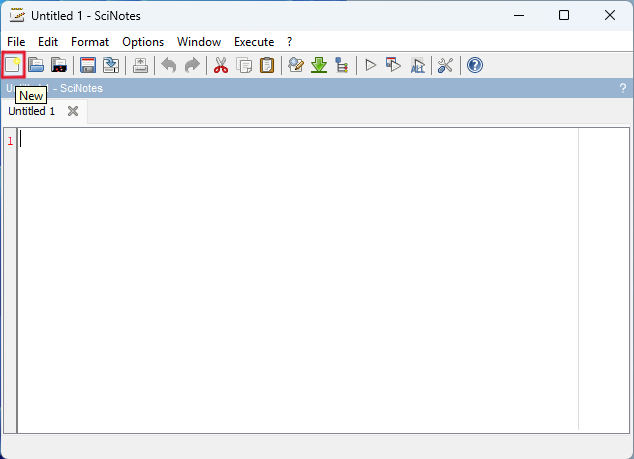
\includegraphics[width=\textwidth,frame]{figures/scinotes/fig_scinotes-new-01.png}
			\end{subfigure}
			\hfill
			\begin{subfigure}[b]{0.48\textwidth}
				\centering
				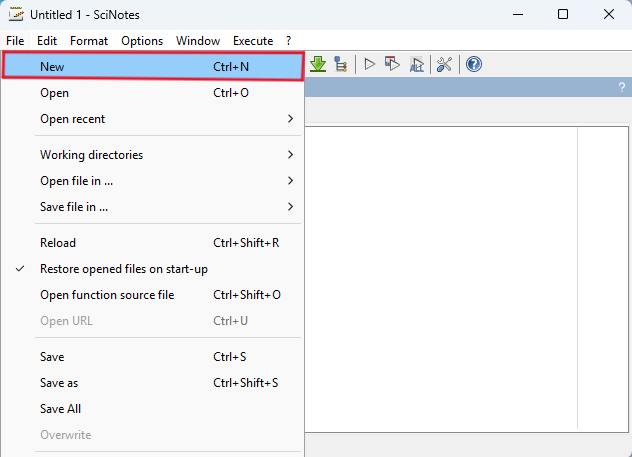
\includegraphics[width=\textwidth,frame]{figures/scinotes/fig_scinotes-new-02.png}
			\end{subfigure}
			\caption{Two ways to create a new script in SciNotes}
			\label{fig:scinotes-new}
		\end{figure}
		
	\subsection{Saving a script}
		Once a Scilab script has been written, it can be saved as follows:
		\begin{enumerate}[I.]
			\item Clicking on the \verb|Save| button on the toolbar or click on \verb|File > Save| from the main menu in Scilab.
			\item Enter a file name, appended with either \verb|.sce| or \verb|.sci| in the file save dialog and then click the \verb|Save| button.
		\end{enumerate}
		These steps are illustrated in figure \ref{fig:scinotes-save}.
		
		\begin{figure}[!h]
			\centering
			\begin{subfigure}[b]{0.48\textwidth}
				\centering
				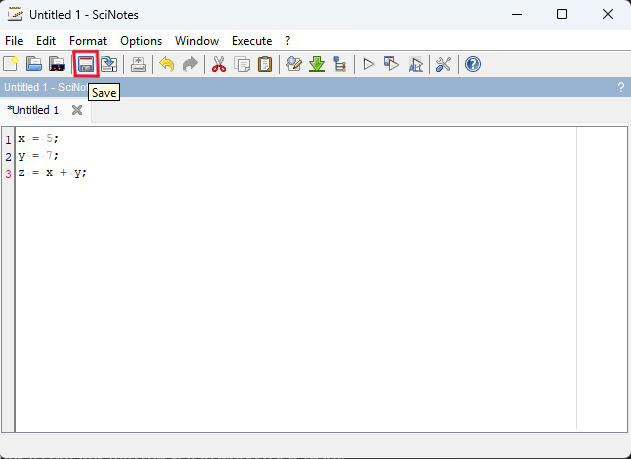
\includegraphics[width=\textwidth,frame]{figures/scinotes/fig_scinotes-save-01.png}
			\end{subfigure}
			\hfill
			\begin{subfigure}[b]{0.48\textwidth}
				\centering
				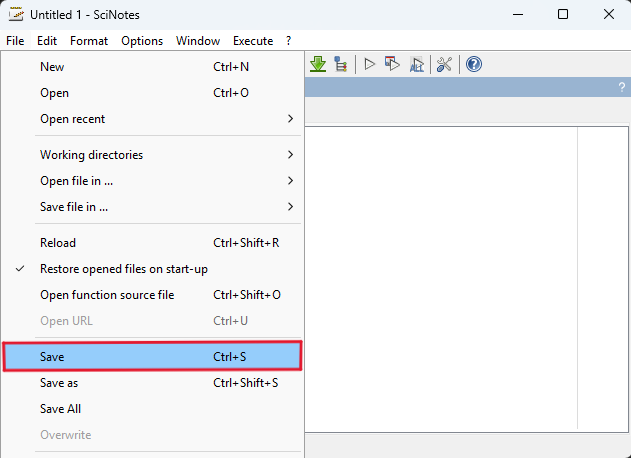
\includegraphics[width=\textwidth,frame]{figures/scinotes/fig_scinotes-save-02.png}
			\end{subfigure}\\ \vspace{2.5ex}
			\begin{subfigure}[b]{0.48\textwidth}
				\centering
				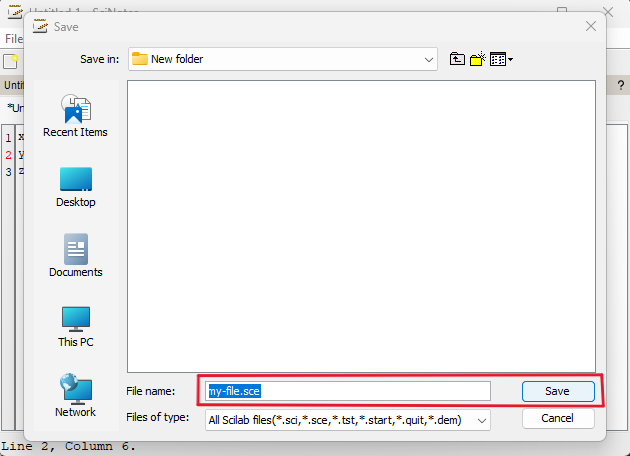
\includegraphics[width=\textwidth,frame]{figures/scinotes/fig_scinotes-save-03.png}
			\end{subfigure}
			\caption{Saving a script in SciNotes}
			\label{fig:scinotes-save}
		\end{figure}
	
	\subsection{Executing a script}
		To execute a script in Scilab, we can click any of the following buttons:
		\begin{enumerate}
			\item The \verb|Execute| button which would execute the current file if the changes are already saved.
			\item The \verb|Save and execute| button which first saves the current file and then executes the same.
			\item The \verb|Save and execute all| button which first saves all the files open as tabs and then executes all of them.
		\end{enumerate}
		The locations of the above buttons in the toolbar are shown in figure \ref{fig:scinotes-execute}.
	
		\begin{figure}[!h]
			\centering
			\begin{subfigure}[b]{0.3\textwidth}
				\centering
				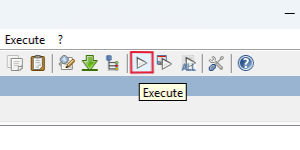
\includegraphics[width=\textwidth,frame]{figures/scinotes/fig_scinotes-execute-01.png}
			\end{subfigure}
			\hfill
			\begin{subfigure}[b]{0.3\textwidth}
				\centering
				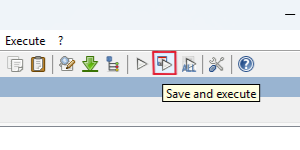
\includegraphics[width=\textwidth,frame]{figures/scinotes/fig_scinotes-execute-02.png}
			\end{subfigure}
			\hfill
			\begin{subfigure}[b]{0.3\textwidth}
				\centering
				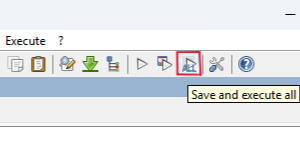
\includegraphics[width=\textwidth,frame]{figures/scinotes/fig_scinotes-execute-03.png}
			\end{subfigure}
			\caption{Executing a script in SciNotes}
			\label{fig:scinotes-execute}
		\end{figure}
		
		An alternate and more flexible way to execute a script in Scilab is by using the \verb|exec()| function which takes the path to a file and executes its contents sequentially. For instance, to execute a Scilab script named \verb|sample-script.sce| which is saved on the Desktop, we can run the following command in the Scilab console:
		\begin{verbatim}
		exec('C:\Users\Desktop\sample-script.sce')
		\end{verbatim}
		The above command would execute the script by echoing all the lines in the script. To suppress this echo, we can run the \verb|exec()| command with an additional \verb|-1| argument:
		\begin{verbatim}
			exec('C:\Users\Desktop\sample-script.sce', -1)
		\end{verbatim}
		
		The practical advantage of the \verb|exec()| over the SciNotes menu is that it can be typed directly at the console, chained with other commands, or embedded inside another script. For instance, one script that loads a shared set of function definitions from a \verb|.sci| file with \verb|exec()| before getting on with its own calculation.